\documentclass[12pt]{beamer}
\usepackage[T2A]{fontenc}
\usepackage[utf8]{inputenc}
\usepackage[english,russian]{babel}
\usepackage{amssymb,amsfonts,amsmath,mathtext}
\usepackage{cite,enumerate,float,indentfirst}
\usepackage{wrapfig} % Text wrapping around figures
%\usepackage{pscyr} % Нормальные шрифты

\graphicspath{{images/}}

\usetheme{Singapore}
%\usecolortheme{whale}

\setbeamertemplate{navigation symbols}{} %remove navigation symbols at all
\setbeamercolor{footline}{fg=black}
\setbeamerfont{footline}{size=\fontsize{8}{10}\selectfont}
\setbeamersize{text margin left=0.6cm, text margin right=0.4cm}
\setbeamertemplate{footline}{
  \leavevmode%
  \hbox{%
%    \begin{beamercolorbox}[wd=.5\paperwidth,ht=2.5ex,dp=1ex,left]{}%
%      Я. А. Воронцов, ВГУ
%    \end{beamercolorbox}%
    \begin{beamercolorbox}[wd=\paperwidth,ht=2.5ex,dp=1ex,right]{}%
      \insertframenumber{} / \inserttotalframenumber \hspace*{2ex}
    \end{beamercolorbox}
  }%
  \vskip0pt%
}

\newcommand{\itemi}{\item[\checkmark]}

\title{\Large{Математическое моделирование задач выбора с расплывчатой неопределенностью на основе методов представления и алгебры нечетких параметров}}
\author{\normalsize{%
Я. А. Воронцов\\%
\emph{Научный руководитель:}~М.Г.Матвеев,~д.т.н.,~профессор.}\\%
\small{
\vspace{2pt}
Специальность 05.13.18~--- математическое моделирование,\\ численные методы и комплексы программ \\
\vspace{2pt}
ФГБОУ ВПО <<Воронежский государственный университет>>%
\vspace{10pt}%
}
\small{Воронеж, 2015}
}

\begin{document}

\maketitle

%%%%%%%%%%%%%%%%%%%%%%%%%%%%%% 2

\begin{frame}
  \frametitle{Представление нечёткой информации}
  \begin{itemize}
    \item нечёткие множества (подмножества предопределённого универсального множества X)
      \begin{equation}
      	\tilde{A}=\left\{ \left( x, \mu_{\tilde A}\left( x \right) \right)\left| x\in X \right. \right\};\ E \left( \mu_{\tilde A} \left( x \right) \right) = \left[0; 1 \right]
      \end{equation}      
    \item нечёткие числа (подмножества множества $\mathbb{R}$)
      \begin{itemize}
        \item кусочная непрерывность $\mu_{\tilde A}\left( x \right)$;
        \item выпуклость $\mu_{\tilde A}\left( x \right)$
      	\begin{gather}
      	  \forall x_1, x_2 \in \mathbb{R}; \forall \gamma \in \left[ 0;1 \right] \notag \\
      	  \mu_{\tilde A}\left( \gamma x_1+\left( 1-\gamma  \right)x_2 \right)\geqslant \min \left\{ \mu_{\tilde A}\left( x_1 \right),\mu_{\tilde A}\left( x_2 \right) \right\}
      	\end{gather}
      	\item нормальность $\mu_{\tilde A}\left( x \right)$
        	\begin{equation}
        		\underset{x\in \mathbb{R}}{\mathop {\sup}}{}\, \left( \mu_{\tilde A} \left( x \right) \right)=1
        	\end{equation}
      \end{itemize}
  \end{itemize}
\end{frame}


%%%%%%%%%%%%%%%%%%%%%%%%%%%%%% 3

\begin{frame}
  \frametitle{Классификация нечётких моделей}
  \begin{columns}[onlytextwidth]
    \begin{column}{0.6\textwidth}
      \begin{figure}[h]
        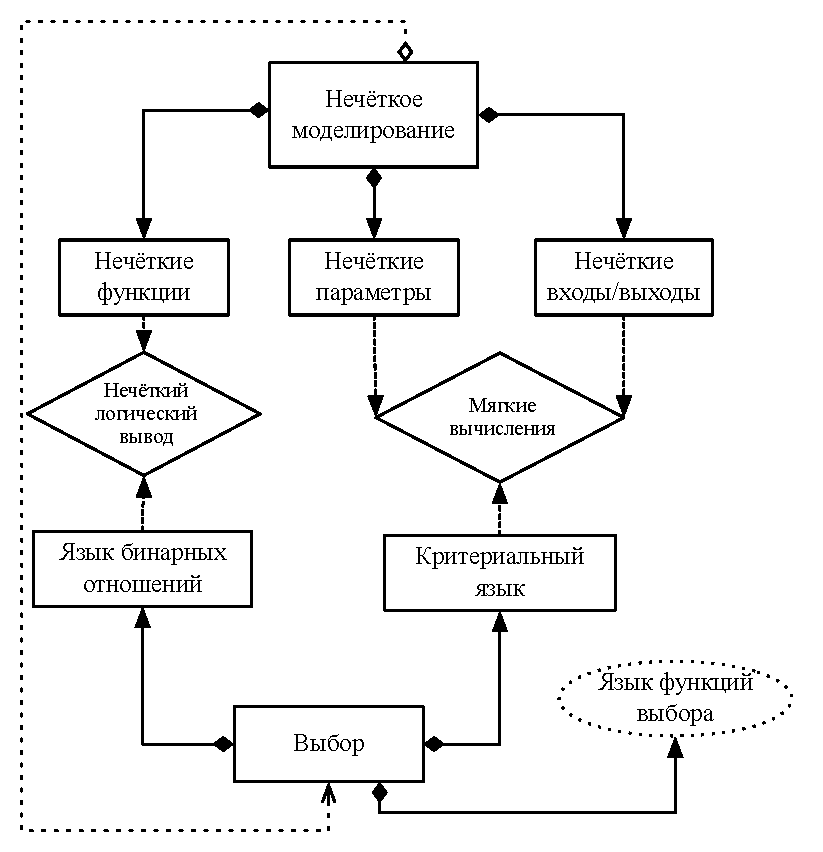
\includegraphics[width=\textwidth]{choice-classification}
      \end{figure}
    \end{column}
    \begin{column}{0.4\textwidth}
      \begin{itemize}
        \item Исследуются модели, использующие чёткие отношения и нечёткие параметры (модели второго типа)
        \item Существующие подходы к нечётким вычислениям далеко не всегда применимы в моделях второго типа
      \end{itemize}
    \end{column}
  \end{columns}
\end{frame}


%%%%%%%%%%%%%%%%%%%%%%%%%%%%%% 4

\begin{frame}
  \frametitle{Особенности существующих способов мягких вычислений}
  \begin{itemize}
    \item требуются значительные вычислительные ресурсы (Ротштейн)
    \begin{gather*}
      \tilde y = f \left(\tilde x_1 \ldots \tilde x_n \right) \rightarrow N = O\left( k^n \right)
    \end{gather*}
    
    \item неоправданно расширяется носитель функции принадлежности
\begin{equation*}
	\begin{matrix}
		\left[ 2;4 \right]\cdot \left[ 1;3 \right]=\left[ 2;12 \right];\quad d=12-2=10; \\ 
		\left[ 2;4 \right]\cdot \left[ 99;101 \right]=\left[ 198;404 \right];\quad d=404-198=206.
	\end{matrix}
\end{equation*}

    \item происходит выход за класс используемых в арифметике чисел из-за искажения формы функции принадлежности;
    \begin{gather*}
      \tilde{C}=\tilde{A}*\tilde{B}=\int\limits_{x_{{\tilde{C}}}^{L}}^{{{m}_{{\tilde{C}}}}}{\frac{{{\mu }_{{\tilde{C}}}}\left( x \right)}{x}}+\int\limits_{{{m}_{{\tilde{C}}}}}^{x_{{\tilde{C}}}^{R}}{\frac{{{\mu }_{{\tilde{C}}}}\left( x \right)}{x}}; \quad 
      \mu_{\tilde C}\left( x \right)=k\sqrt{x}+b
    \end{gather*}

  \end{itemize}
\end{frame}

%%%%%%%%%%%%%%%%%%%%%%%%%%%%%% 5

\begin{frame}
  \frametitle{Особенности существующих способов мягких вычислений}
  \begin{itemize}
    \item ограничивается область определения функции принадлежности
    \begin{gather*}
      \tilde A = \left( {{m}_{1}},{{a}_{1}},{{b}_{1}} \right); \quad \tilde B = \left( {{m}_{2}},{{a}_{2}},{{b}_{2}} \right); \\
      \tilde A \times \tilde B=\left( {{m}_{1}}{{m}_{2}},{{m}_{2}}{{a}_{1}}+{{m}_{1}}{{a}_{2}},{{m}_{2}}{{b}_{1}}+{{m}_{1}}{{b}_{2}} \right);\quad \tilde A, \tilde B > 0\\
      \tilde A \times \tilde B =\left( {{m}_{1}}{{m}_{2}},{{m}_{2}}{{a}_{1}}-{{m}_{1}}{{b}_{2}},{{m}_{2}}{{b}_{1}}-{{m}_{1}}{{a}_{2}} \right); \quad \tilde A> 0, \tilde B < 0\\
      \tilde A \times \tilde B=\left( {{m}_{1}}{{m}_{2}},-{{m}_{2}}{{b}_{1}}-{{m}_{1}}{{b}_{2}},-{{m}_{2}}{{a}_{1}}-{{m}_{1}}{{a}_{2}} \right); \quad \tilde A, \tilde B < 0
    \end{gather*}
    \item нарушаются классические отношения равенства и частичного порядка.
    \begin{gather*}
      \left( \tilde A + \tilde B \right) - \tilde B \neq \tilde A
    \end{gather*}

  \end{itemize}
\end{frame}


%%%%%%%%%%%%%%%%%%%%%%%%%%%%%% 6

\begin{frame}
  \frametitle{Цель и задачи исследования}
  \textbf{Цель:} построение и исследование моделей учёта нечёткой неопределённости, обеспечивающих требуемые свойства решения (ограничение роста неопределённости, сохранение истинности модельных отношений, устойчивость решения) различных прикладных задач, а также разработка методов эффективного численного решения на основе вводимых моделей \\
  \textbf{Задачи:}
  \begin{itemize}
    \item анализ существующих методик нечётких вычислений с~точки зрения сохранения свойств решения задач;
    \item разработка модели представления нечётких чисел, позволяющей максимально сохранять исходную экспертную информацию и обеспечить требуемые качественные свойства решений (устойчивость, сохранение чётких математических соотношений и т.\,п.);
  \end{itemize}  
\end{frame}

%%%%%%%%%%%%%%%%%%%%%%%%%%%%%% 7

\begin{frame}
  \frametitle{Цель и задачи исследования}
  \textbf{Задачи:}
  \begin{itemize}
    \item разработка методики эффективной численной реализации решения задач с нечёткими параметрами, основанной на подходящих алгебраических структурах и её тестирование на примере задачи сетевого планирования с нечёткими параметрами;
    \item разработка и верификация программного обеспечения, реализущего предложенную модель представления нечётких параметров и методики численного решения задач с нечёткими параметрами.
  \end{itemize}  
\end{frame}


%%%%%%%%%%%%%%%%%%%%%%%%%%%%%% 8

\begin{frame}
  \frametitle{Основные понятия}
  \begin{itemize}
    \item Треугольное нечёткое число $\tilde A = \left\langle m,a,b \right\rangle $
      \begin{equation}
        \mu_{\tilde A}\left( x \right)=
        \left\{ \begin{aligned}
			& \frac{x-m+a}{a};\ x\in \left[ m-a;m \right] \\ 
			& \frac{m+b-x}{b};\ x\in \left( m;m+b \right] \\ 
			& 0;\ \text{в остальных случаях} 
	 	\end{aligned} \right.
      \end{equation}
    \item Горизонтальная форма (Пегат) $X_\alpha = \left[x^L(\alpha); x^R(\alpha) \right]$
      \begin{equation}
        \left[ 
          \begin{aligned}
            & x^L(\alpha )=m-a+a\alpha  \\ 
            & x^R(\alpha )=m+b-b\alpha
          \end{aligned}
        \right.
      \end{equation}
    \item Треугольное число $LL$ $\left( RR \right)$-типа~--- правый (левый) коэффициент нечёткости числа равен нулю
  \end{itemize}
\end{frame}

%%%%%%%%%%%%%%%%%%%%%%%%%%%%%% 9

\begin{frame}
  \frametitle{Преобразование L}
  \begin{itemize}
    \item Переход к интервальной неопределенности
      \begin{equation}
        \label{eq:task-transform}
      	\tilde{Y} = f\left( \tilde X, \tilde A \right)\to \bigcup\limits_{\alpha =0}^{1}{y_\alpha}=f\left( X_\alpha, A_\alpha \right)
      \end{equation}
    \item Формализованное представление $\alpha$-интервала с помощью преобразования $L$
      \begin{equation}
        \label{eq:L-transform-base}
        \bar{x}\left( \alpha  \right)=L\left( X_\alpha \right)=\lambda x^L \left( \alpha  \right)+\left( 1-\lambda  \right) x^R \left( \alpha  \right);\, \lambda \in \left[0; 1 \right]
      \end{equation}
    \item Синтез модифицированного решения
      \begin{equation}
        \tilde Y^{*}= \bigcup\limits_{\alpha =0}^{1} f\left(L\left( X_\alpha \right), L\left( A_\alpha \right) \right)=\left\{ y_\alpha \left| \mu_{\tilde Y^*}(y)=\alpha \right. \right\}
      \end{equation}
    \item Модифицированное нечёткое число (LL/RR-типа)
      \begin{equation}
        \label{eq:modified-number}
        \mu_{\tilde A^{*}}\left( x \right)={\left( \bar{x}\left( \alpha  \right) \right)}^{-1}
      \end{equation}
  \end{itemize}
\end{frame}

%%%%%%%%%%%%%%%%%%%%%%%%%%%%%% 10

\begin{frame}
  \frametitle{Преобразование L}
  \begin{figure}
    \center
    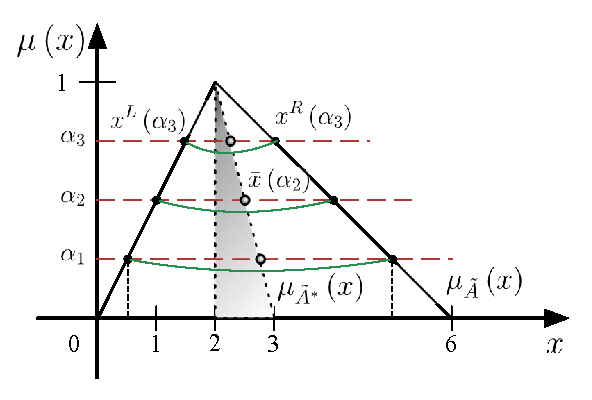
\includegraphics[width=\textwidth]{l-transform-full}
  \end{figure}
\end{frame}

%%%%%%%%%%%%%%%%%%%%%%%%%%%%%% 11

\begin{frame}
  \frametitle{Представление числа}
  \begin{itemize}
    \item Вводится модель представления нечёткого числа, инвариантноя к его расположению на числовой оси  $\left\langle m_{\tilde A}, d_{\tilde A}, AS_{\tilde A} \right\rangle$; $d_{\tilde A} = a+b$; $\displaystyle AS_{\tilde A} = \frac{b-a}{2}$.
  \end{itemize}
  \begin{figure}[h]
    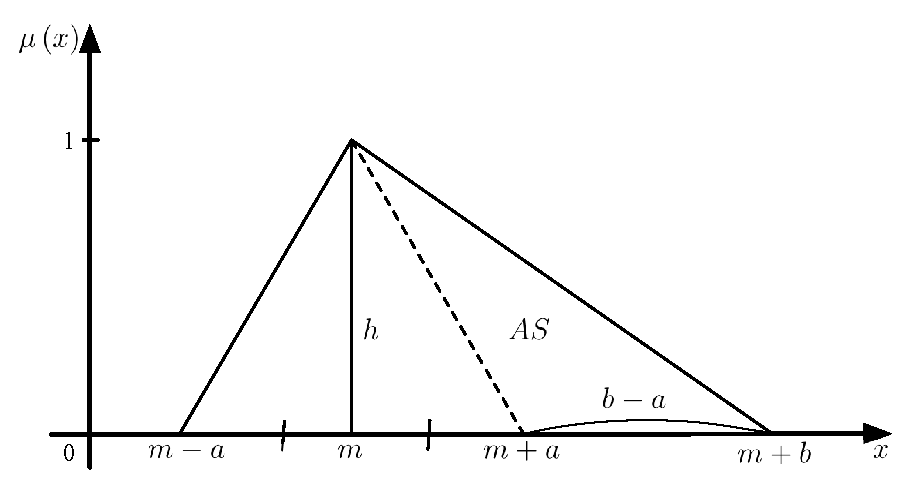
\includegraphics[width=0.9\textwidth]{as-degree}
  \end{figure}
\end{frame}

%%%%%%%%%%%%%%%%%%%%%%%%%%%%%% 12

\begin{frame}
  \frametitle{Свойства преобразования L}
  \begin{enumerate}
    \item Преобразование $L$ сохраняет моду нечёткого числа, т.\,е. $\forall \lambda \in \left[ 0;1 \right]:\ m_{\tilde A}=m_{\tilde A^{*}}$.
    \item При некоторых значениях параметра $\lambda$ преобразование $L$ сохраняет
      \begin{enumerate}
        \item знак степени асимметрии: $\exists \lambda \in [0;1]:\ sign(AS_{\tilde A})=sign(AS_{\tilde A^{*}})$;
        \item значение степени асимметрии: $\exists \lambda \in [0;1]:\ AS_{\tilde A}=AS_{\tilde A^{*}}$.
      \end{enumerate}
      $\displaystyle \lambda^* =\frac{a}{a+b}=\frac{a}{d_{\tilde A}}$ сохраняет значение степени асимметрии.
    \item $\forall \lambda \in \left[ 0;1 \right]: A_{\alpha}^{*}\subset A_\alpha;\ d_{\tilde A} \geqslant d_{\tilde A^{*}}$~--- преобразование~$L$ уменьшает длину носителя нечёткого числа и~оставляет $\alpha$-интервалы модифицированного числа внутри $\alpha$-интервалов исходного числа.
  \end{enumerate}
\end{frame}

%%%%%%%%%%%%%%%%%%%%%%%%%%%%%% 13

\begin{frame}
  \frametitle{Алгебра модифицированных нечётких чисел}
  \begin{itemize}
    \item Aлгебра $P=\left\langle K ;\ +,\,*, 0, 1 \right\rangle$, $K=\left\lbrace \bar x(\alpha) \right\rbrace, \alpha \in \left[0; 1\right]$
      \begin{equation}
        \label{eq:def-one}
        \bar{x}\left( \alpha  \right)=c+k\alpha,
      \end{equation}
    \item Коэффициенты в~\eqref{eq:def-one}
      \begin{equation}
        \label{eq:modified-number-from-abm}
        \begin{aligned}
          & \left[ \begin{aligned}
          & c=m+b-\lambda \left( a+b \right) \\ 
          & k=\lambda \left( a+b \right)-b \\ 
        \end{aligned} \right. \\ 
        & \lambda \in \left[ 0;1 \right];\ c,k\in \mathbb{R} \\ 
      \end{aligned}
      \end{equation}
    \item Элементы множества $K$ линейны; достаточно знать два значения~--- $\bar{x}_{\tilde A}\left( 0 \right)$ и~$\bar{x}_{\tilde A}\left( 1 \right)=m_{\tilde A}$, чтобы найти $\tilde{A}$:
      \begin{gather}
        \label{eq:isomorphic-field}
        \bar{x}_{\tilde A}\left( \alpha \right)=\bar{x}_{\tilde A}\left( 0 \right)+\alpha \left(\bar{x}_{\tilde A}\left( 1 \right)-\bar{x}_{\tilde A}\left(0 \right) \right)=\\
        =\alpha \bar{x}_{\tilde A}\left( 1 \right)+\left( 1-\alpha  \right) \bar{x}_{\tilde A}\left( 0 \right)
      \end{gather}
  \end{itemize}
\end{frame}

%%%%%%%%%%%%%%%%%%%%%%%%%%%%%% 14

\begin{frame}
  \frametitle{Сложение и его свойства}
  \begin{itemize}
    \item Операция сложения на~множестве $K$
      \begin{equation}
        \label{eq:fuzzy-addition}
        \bar{x}_1\left(\alpha \right)+\bar{x}_2\left(\alpha \right)=r_1\left( \alpha  \right)=c_1+c_2+\left(k_1+k_2 \right)\alpha,\ r_1 \left( \alpha  \right)\in K
      \end{equation}
    \item Нейтральный по сложению элемент
      \begin{gather}
        \label{eq:fuzzy-zero}
        \bar{0}=0+0\alpha \in K: \forall \bar{x}(\alpha )\in K: \notag \\ 
        \bar{x}(\alpha )+\bar{0}=c+k\alpha +0+0\alpha =\bar{x}(\alpha )
      \end{gather}
    \item Противоположный по сложению элемент~\eqref{eq:fuzzy-minus} 
      \begin{equation}
        \label{eq:fuzzy-minus}
        -\bar{x}\left(\alpha \right)=-c-k\alpha \in K:\ \bar{x}\left( \alpha  \right)+\left( -\bar{x}\left( \alpha  \right) \right)=\bar{0}
      \end{equation}
    \item Алгебра $\left \langle K,+,0 \right \rangle$~--- абелева группа
  \end{itemize}
\end{frame}

%%%%%%%%%%%%%%%%%%%%%%%%%%%%%% 15

\begin{frame}
  \frametitle{Умножение и его свойства}
  \begin{itemize}
    \item Операция умножения на~множестве $K$
      \begin{equation}
      \label{eq:fuzzy-multiplication}
        r_2\left( \alpha \right)=c_1 c_2+\left(c_1 k_2+ c_2 k_1 +k_1 k_2 \right)\alpha;\ r_2\left( \alpha  \right)\in K
      \end{equation}
    \item Нейтральный по умножению элемент
      \begin{equation}
        \label{eq:fuzzy-one}
        \bar{1}=1+0\alpha \in K:\ \forall \bar{x}\left( \alpha  \right)\in K\quad \bar{x}\left( \alpha  \right)\cdot \bar{1}=\bar{x}\left( \alpha  \right)
      \end{equation}
    \item Обратный по умножению элемент
      \begin{equation}
        \label{eq:fuzzy-division}
        \bar{x}^{-1}(\alpha )=\frac{1}{c}-\frac{k}{c\left(c+k\right)}\alpha \in K,\ c\ne 0:\ \bar{x}\left(\alpha \right){{\bar{x}}^{-1}}\left( \alpha  \right)=\bar{1}
      \end{equation}
    \item При~$c+k=m=0$~\eqref{eq:modified-number-from-abm} обратного элемента для $\bar{x}\left( \alpha  \right)$ не существует
    \item Алгебра обратимых элементов $\left \langle K,*,1 \right \rangle$~--- абелева группа
    \item Умножение дистрибутивно относительно сложения
  \end{itemize}
\end{frame}

%%%%%%%%%%%%%%%%%%%%%%%%%%%%%% 16

\begin{frame}
  \frametitle{Двухточечные вычисления}
  \begin{figure}[h]
    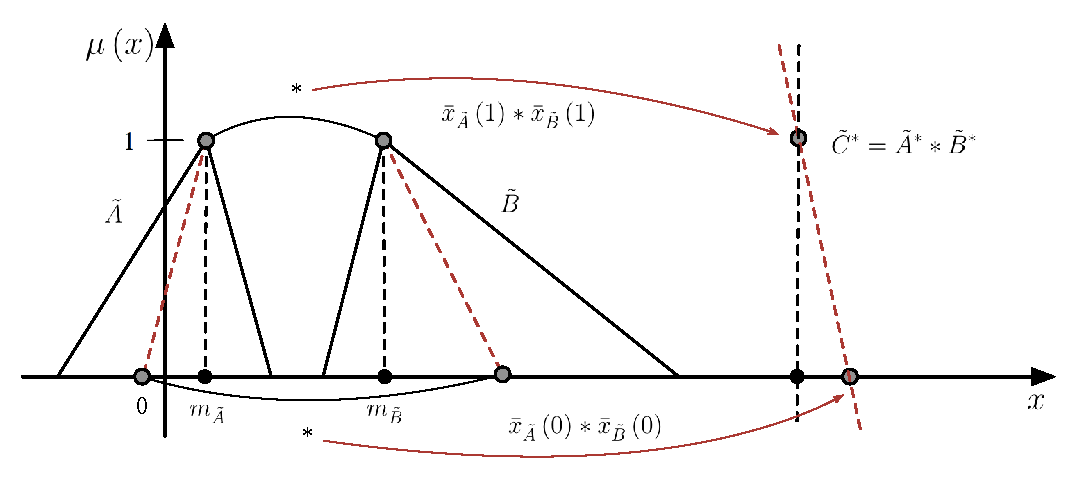
\includegraphics[width=\textwidth]{two-point}
  \end{figure}
  Для произвольной арифметической операции~$g: R^2 \rightarrow R$
  \begin{gather}
    \bar{x}_{\tilde A}\left( \alpha \right)g\bar{x}_{\tilde B}\left(\alpha \right)=\notag\\
    \label{eq:two-point-calculations}
    =\alpha \left(\bar{x}_{\tilde A}\left( 1 \right)g\bar{x}_{\tilde B}\left(1 \right) \right)+\left(1-\alpha \right)\left(\bar{x}_{\tilde A}\left(0 \right)g\bar{x}_{\tilde B}\left(0 \right) \right)
  \end{gather}
\end{frame}

%%%%%%%%%%%%%%%%%%%%%%%%%%%%%% 17

\begin{frame}
  \frametitle{Двухточечные вычисления}
  \begin{itemize}
  \item Cуществуют отображения $\Gamma:\ K \to M$ и $\Gamma^{-1}:\ M \to K$:
\begin{equation}
  \label{eq:isomorph-transition}
  \left[ \begin{aligned}
    & P=\left\langle K, \Omega_1 \right\rangle \\
    & c=\bar{x}_{\tilde A}\left( 0 \right); \\ 
    & k=\bar{x}_{\tilde A}\left( 1 \right)-\bar{x}_{\tilde A}\left( 0 \right);
  \end{aligned} \right.
  \Leftrightarrow 
  \left[ \begin{aligned}
    & Q=\left\langle M, \Omega_2 \right\rangle \\
    & \bar{x}_{\tilde A}\left( 0 \right)=c; \\ 
    & \bar{x}_{\tilde A}\left( 1 \right)=c+k;
  \end{aligned} \right.
\end{equation}
  \item Для бинарных операций $\varphi_i \in \Omega_1$, $\psi_i \in \Omega_2$ и элементов $k_1, k_2 \in K$, $m_1, m_2 \in M$:
\begin{gather}
  \label{eq:gomomorph-1}
  \Gamma\left( \varphi_i \left( k_1, k_2 \right) \right) = \psi_i\left( \Gamma \left(k_1, k_2 \right) \right); \\
  \label{eq:gomomorph-2}
  \varphi_i\left( \Gamma^{-1} \left(m_1, m_2 \right) \right) = \Gamma^{-1}\left( \psi_i \left(m_1, m_2 \right) \right)
\end{gather}
  \item Ввиду \eqref{eq:isomorph-transition}, $K$ и $M$ суть одно и то же~--- изоморфизм доказывается простой подстановкой
  \end{itemize}
\end{frame}

%%%%%%%%%%%%%%%%%%%%%%%%%%%%%% 18

\begin{frame}
  \frametitle{Устойчивость ЗЛП}
  Задача линейного программирования с нечёткими параметрами
    \begin{equation}
      \label{eq:fuzzy-lp-unstable-problem}
      \left\{ \begin{aligned}
        & f\left( \mathbf{x} \right)=\mathbf{Cx}\to \min;  \\ 
        & \mathbf{Ax}=\mathbf{B},
      \end{aligned} \right.
      \to
      \left\{ \begin{aligned}
        & f\left( \mathbf{x} \right)={\mathbf{C}^{*}}\mathbf{x}\to \min;  \\ 
        & {\mathbf{A}^{*}}\mathbf{x}={\mathbf{B}}^{*},
      \end{aligned} \right.
    \end{equation}
    
  \begin{wrapfigure}{r}{0.5\textwidth}
    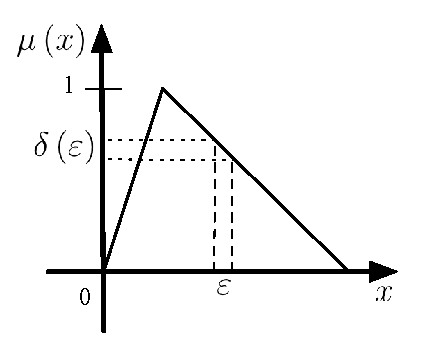
\includegraphics[width=0.4\textwidth]{stability}
  \end{wrapfigure}

  Решение задачи устойчиво (по Тихонову), если
        \begin{gather}
        \forall \varepsilon >0\, \exists \delta >0\, \forall \alpha_1, \alpha_2 \in \left[0; 1\right] \notag \\
        \left| \alpha_1 - \alpha_2 \right|<\delta \Rightarrow   \notag \\
        \label{eq:fuzzy-solution-stability}
        \left\| \mathbf{x}\left( \alpha_1 \right)-\mathbf{x} \left( \alpha_2  \right) \right\|<\varepsilon
        \end{gather}

\end{frame}

%%%%%%%%%%%%%%%%%%%%%%%%%%%%%% 19

\begin{frame}
  \frametitle{Устойчивость ЗЛП}
  \begin{itemize}
    \item При $\alpha=0$, все~значения $\lambda_S$ ($S$~--- индекс $\tilde A_{ij}$, $\tilde B_i$, $\tilde C_i$)~--- принимают граничные значения (0 или 1). 
    \item Ограничения на $\lambda$ для минимизации потерь экспертной информации
      \begin{equation}
      \label{eq:lambda-minimization-criterion}
        {\left( \lambda_{S}^{\star}-\lambda_S \right)}^2\to \min
      \end{equation}
    \item Задача векторной оптимизации ввиду противоречивости критерия~\eqref{eq:lambda-minimization-criterion} и~целевой~функции задачи~\eqref{eq:fuzzy-lp-unstable-problem}
    \item Применяется аддитивная свёртка критериев в~целевой функции~\eqref{eq:modified-target-function}
      \begin{equation}
      \label{eq:modified-target-function}
        f^{*}\left( \mathbf{x}, \lambda \right)=\mathbf{C}^{*}\mathbf{x}+\gamma \sum\limits_{s}^{}{\left(\lambda_{S}^{*}-\lambda_S \right)}^{2} \to \min
      \end{equation}
  \end{itemize}
\end{frame}

%%%%%%%%%%%%%%%%%%%%%%%%%%%%%% 20

\begin{frame}
  \frametitle{Задача сетевого планирования}
  \begin{figure}
    \center
    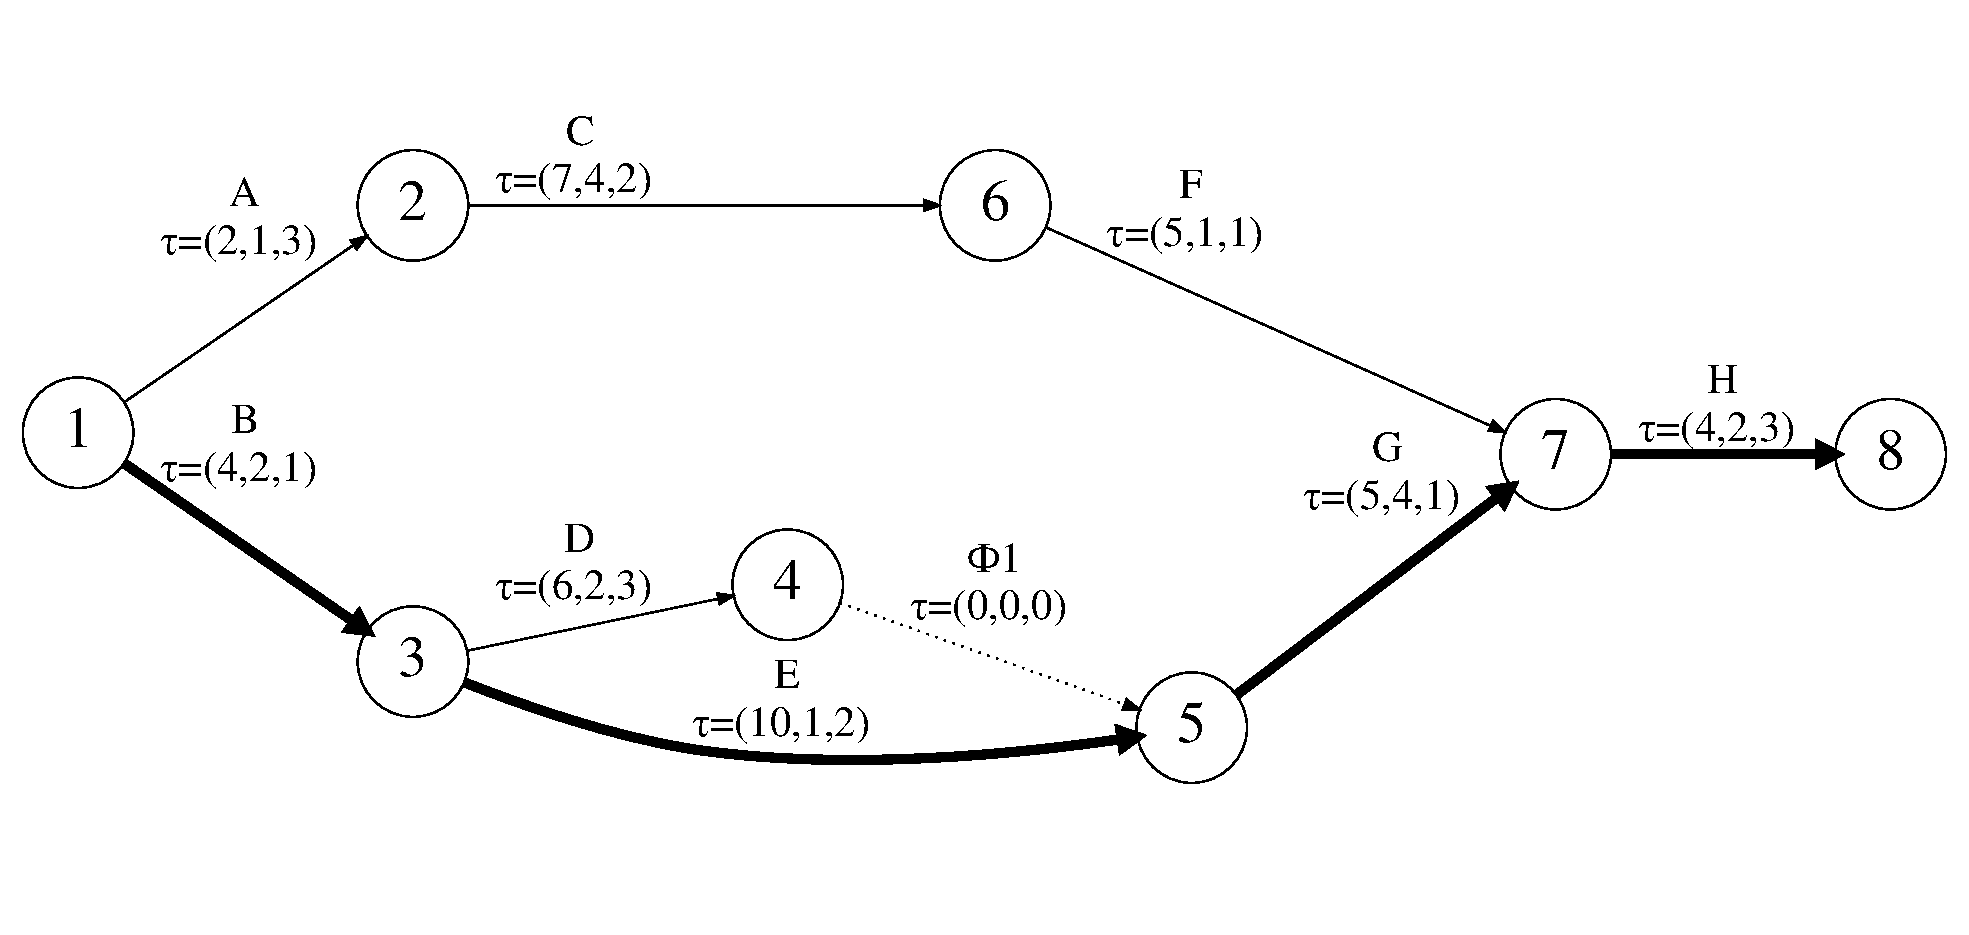
\includegraphics[width=\textwidth]{pplan}
  \end{figure}
  $G=(V,E)$, $\left| V \right|=n$, $\left| E \right|=m$; \\
  дуги $e_j$~--- работы $w_j$, длительностью $\tau_j$, $j=\overline{1,m}$; \\
  вершины $v_i$~--- события $z_i$ с~временами наступления $t_i$, $i=\overline{1,n}$
\end{frame}

%%%%%%%%%%%%%%%%%%%%%%%%%%%%%% 21

\begin{frame}
  \frametitle{Модифицированная задача сетевого планирования}
  \begin{itemize}
    \item ЗЛП с~нечёткими временными оценками
      \begin{equation}
      \label{eq:modified-fcpm-lp}
        \left\{ \begin{aligned}
          & T(\alpha )=t_n-t_1\to \min  \\ 
          & t_{j_s}-t_{i_s}\geqslant \bar{\tau}_s\left(\alpha,\lambda_s \right),\ \forall s=\overline{1,m}.
        \end{aligned} \right.
      \end{equation}
    \item При $\alpha = 0$ решается возмущённая задача
      \begin{equation}
      \label{eq:modified-fcpm-lp-alpha}
        \left \{ \begin{aligned}
          & T^* \left(\alpha, \lambda \right) = t_n-t_1+\gamma \sum \limits_{s=1}^{m} \left(\lambda_s^*-\lambda_s \right)^2 \to \min; \\
          & t_{j_{s_1}}-t_{i_{s_1}} = \bar{\tau}_{s_1}\left(\alpha, \lambda_{s_1} \right),\ \forall s_1 \in S_1\left(1\right); \\
          & t_{j_s}-t_{i_s} \geqslant \bar{\tau}_s\left(\alpha, \lambda_s \right),\ \forall s \notin S_1\left(1\right),\,s=\overline{1,m}.
        \end{aligned} \right.
      \end{equation}
    \item Результат~--- совокупность $\left \langle \tilde T, S_1, \lambda \right \rangle$
  \end{itemize}
\end{frame}

%%%%%%%%%%%%%%%%%%%%%%%%%%%%%% 22

\begin{frame}
  \frametitle{Решение примера (с. 19)}
  \begin{figure}
    \center
    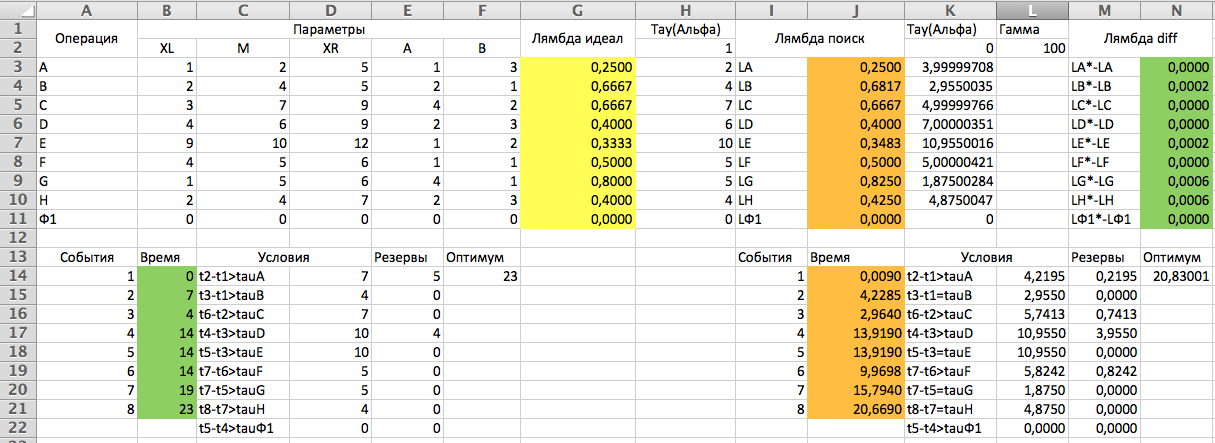
\includegraphics[width=\textwidth]{excel-screen.png}
  \end{figure}
  Окончательный результат: $S_1=\left\{ B,E,G,H \right\}$, $T\left( \alpha \right)=20,67+2,33\alpha$, $\lambda =\left\{ 0,25;\ 0,68;\ 0,67;\ 0,4;\ 0,35;\ 0,5;\ 0,83;\ 0;43 \right\}$
\end{frame}

%%%%%%%%%%%%%%%%%%%%%%%%%%%%%% 23

\begin{frame}
  \frametitle{Программное обеспечение}
  \begin{figure}
    \center
    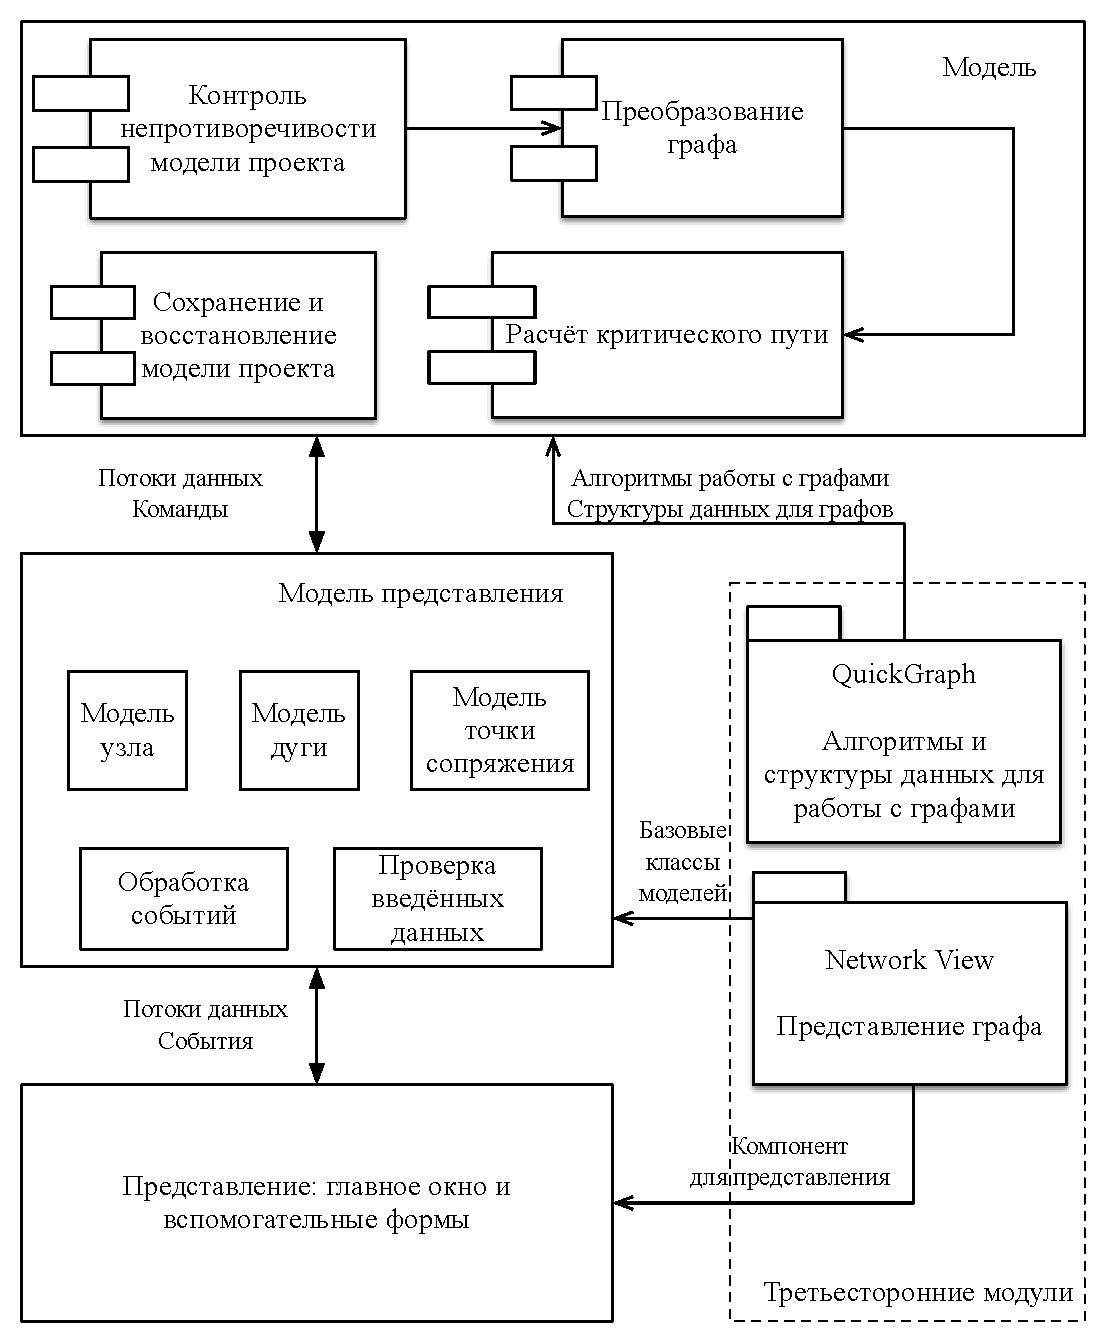
\includegraphics[width=0.55\textwidth]{app-architecture}
  \end{figure}
\end{frame}

%%%%%%%%%%%%%%%%%%%%%%%%%%%%%% 24

\begin{frame}
  \frametitle{Результаты работы (мат. моделирование)}
  \begin{itemize}
  \item Разработана и исследована модель представления нечётких числовых параметров математического описания объектов в классе треугольных LR-чисел, обеспечивающая возможность построения алгебраической структуры нечётких чисел, сохраняющей требуемые свойства решения задач выбора: ограничение роста неопределённости, сохранение истинности модельных отношений и возможность интерпретации полученного результата.
  \end{itemize}
\end{frame}

%%%%%%%%%%%%%%%%%%%%%%%%%%%%%% 25

\begin{frame}
  \frametitle{Результаты работы (численные методы)}
  \begin{itemize}
    \item Разработан метод приближённого численного решения задач выбора с нечёткими параметрами, инвариантный к форме математического описания задачи, позволяющий строить нечёткое решение задач как линейную комбинацию чётких решений, полученных на границах интервального представления параметров, снизить вычислительную сложность процесса получения решения и применять стандартные программные продукты для нечётких вычислений.
  \end{itemize}
\end{frame}

%%%%%%%%%%%%%%%%%%%%%%%%%%%%%% 26

\begin{frame}
  \frametitle{Результаты работы (апробация методов)}
  \begin{itemize}
  \item Предложенные методы решения задач выбора с нечёткими параметрами апробированы на задаче сетевого планирования с нечёткими временными оценками. В процессе апробации рассмотрена проблема устойчивости критического пути, обосновано введение свёртки критериев для управления устойчивостью и сформулирован алгоритм, обеспечивающий получение устойчивого решения задачи. Достоверность полученного решения подтверждается его сравнением с решениями, найденным с помощью других методов, хорошо зарекомендовавших себя в мировой практике.
  \end{itemize}
\end{frame}

%%%%%%%%%%%%%%%%%%%%%%%%%%%%%% 27

\begin{frame}
  \frametitle{Результаты работы (комплексы программ)}
  \begin{itemize}
    \item Разработан программный комплекс, позволяющий решать задачу оценки сроков при разработке программного обеспечения как задачу сетевого планирования с нечёткими временными оценками и обеспечивающий учёт возможных рисков, возникающих при разработке программного обеспечения. Практическая ценность коплекса подтверждается актом о внедрении.   
  \end{itemize}
\end{frame}

%%%%%%%%%%%%%%%%%%%%%%%%%%%%%% 28

\begin{frame}
  \frametitle{Апробация работы и публикации}
  Основные положения работы докладывались на конференциях:
  \begin{itemize}
    \item Современные проблемы прикладной математики, теории управления и математического моделирования (Воронеж, 2012 г.)
    \item Информатика: проблемы, методология, технологии (Воронеж, 2013--2014 гг.);
    \item Современные технологии в задачах управления, автоматики и обработки информации (Алушта, 2013--2014 гг.);
    \item Радиоэлектроника, электротехника и энергетика (Москва, 2014).
  \end{itemize}
  Основное содержание диссертационного исследования изложено в 11 научных работах, из~них 4 статьи в~изданиях, рекомендованных ВАК РФ.
\end{frame}

\end{document} 